\chapter{Analisis dan Perancangan}

\section{Analisis Malware WannaCry}

Pada bagian ini, peneliti memfokuskan analisa malware WannaCry pada analisa lalu lintas paket yang dilakukan oleh host terinfeksi dengan melakukan machine-in-the-middle. Analisis malware WannaCry dilakukan dengan melakukan \textit{sniffing} dengan menggunakan 3 host dengan jaringan terisolasi seperti pada gambar \ref{fig:analisis_malware_net}. 
Ketiga host tersebut memiliki arsitektur yang sama yakni x86\_64 sehingga tidak ada alignment (seperti little endian dan big endian) berbeda.

\begin{figure}[H]
	\centering
	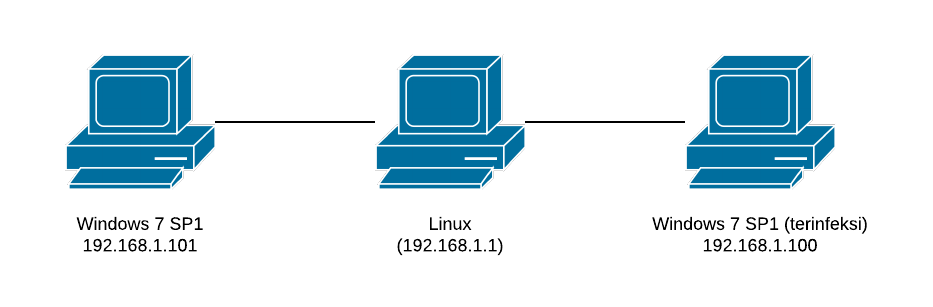
\includegraphics[width=400px]{resources/analisis_malware_net.png}
	\caption{Susunan jaringan untuk analisis malware WannaCry}
	\label{fig:analisis_malware_net}
\end{figure}

Host linux (192.168.1.1) menjadi host dengan dua interface yang dijadikan \textit{bridge}. Sehingga host Windows 7 terinfeksi (192.168.1.100) dapat berkomunikasi dengan host Windows 7 SP1 (192.168.1.101) hanya melalui 192.168.1.1. Kemudian pada host linux dilakukan sniffing dengan menggunakan tcpdump. dengan command sebagai berikut:

\begin{verbatim}
$ tcpdump -s0 -i br0 -vv -w output.wannacry-1.pcap
\end{verbatim}

\section{Karakteristik Malware WannaCry}

Dari pengelompokan malware menjadi worm, virus dan trojan horse menurut (\cite{idika2007survey}) maka WannaCry digolongkan sebagai worm. Sesuai dengan karakteristik yang disebutkan WannaCry memiliki kapabilitas menginfeksi melalui network. WannaCry memiliki dua buah bagian utama: ransomware, dan worm penginfeksi, yang melakukan penyebaran melalui protokol SMB. Jika sebuah host hanya menjalankan bagian ransomware saja, maka tidak akan ada penyebaran yang dilakukan, seperti ditunjukan pada Gambar \ref{fig:no_infect_action}.

Sedangkan jika host menjalankan bagian dropper, dropper tersebut akan menjalankan worm penginfeksi dan sekaligus menjalankan ransomware. Pada Gambar \ref{fig:infect_action} terlihat host 192.168.1.100  mencoba melakukan koneksi ke port \verb|445/tcp| setiap host yang berada pada subnet yang sama.

\begin{figure}[H]
	\centering
	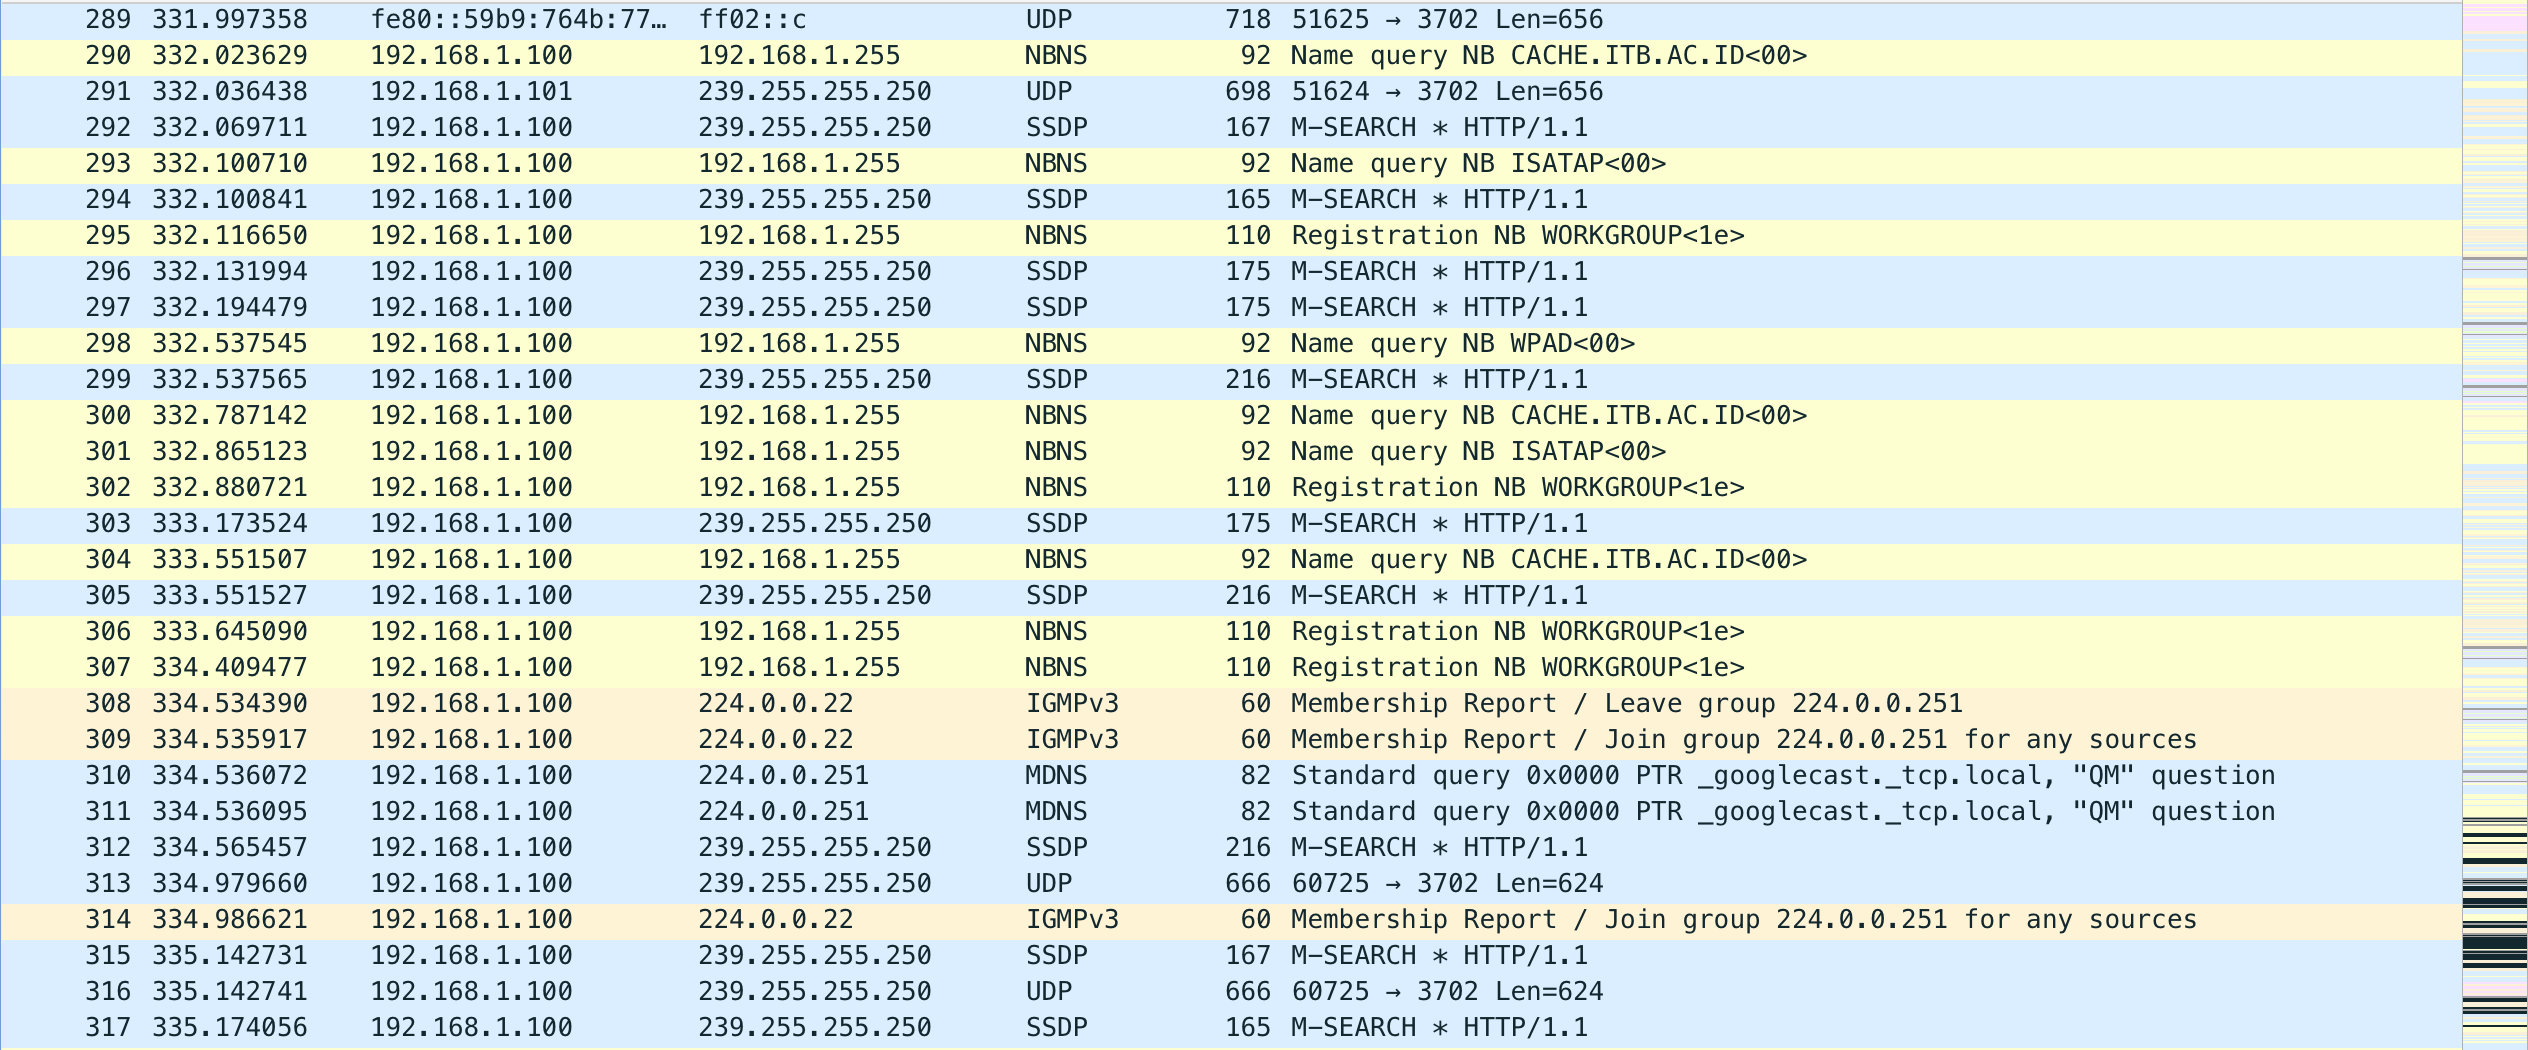
\includegraphics[width=\textwidth]{resources/no_infect_action.png}
	\caption{Paket pada host terinfeksi ransomware tanpa worm penginfeksi}
	\label{fig:no_infect_action}
\end{figure}

\begin{figure}[H]
	\centering
	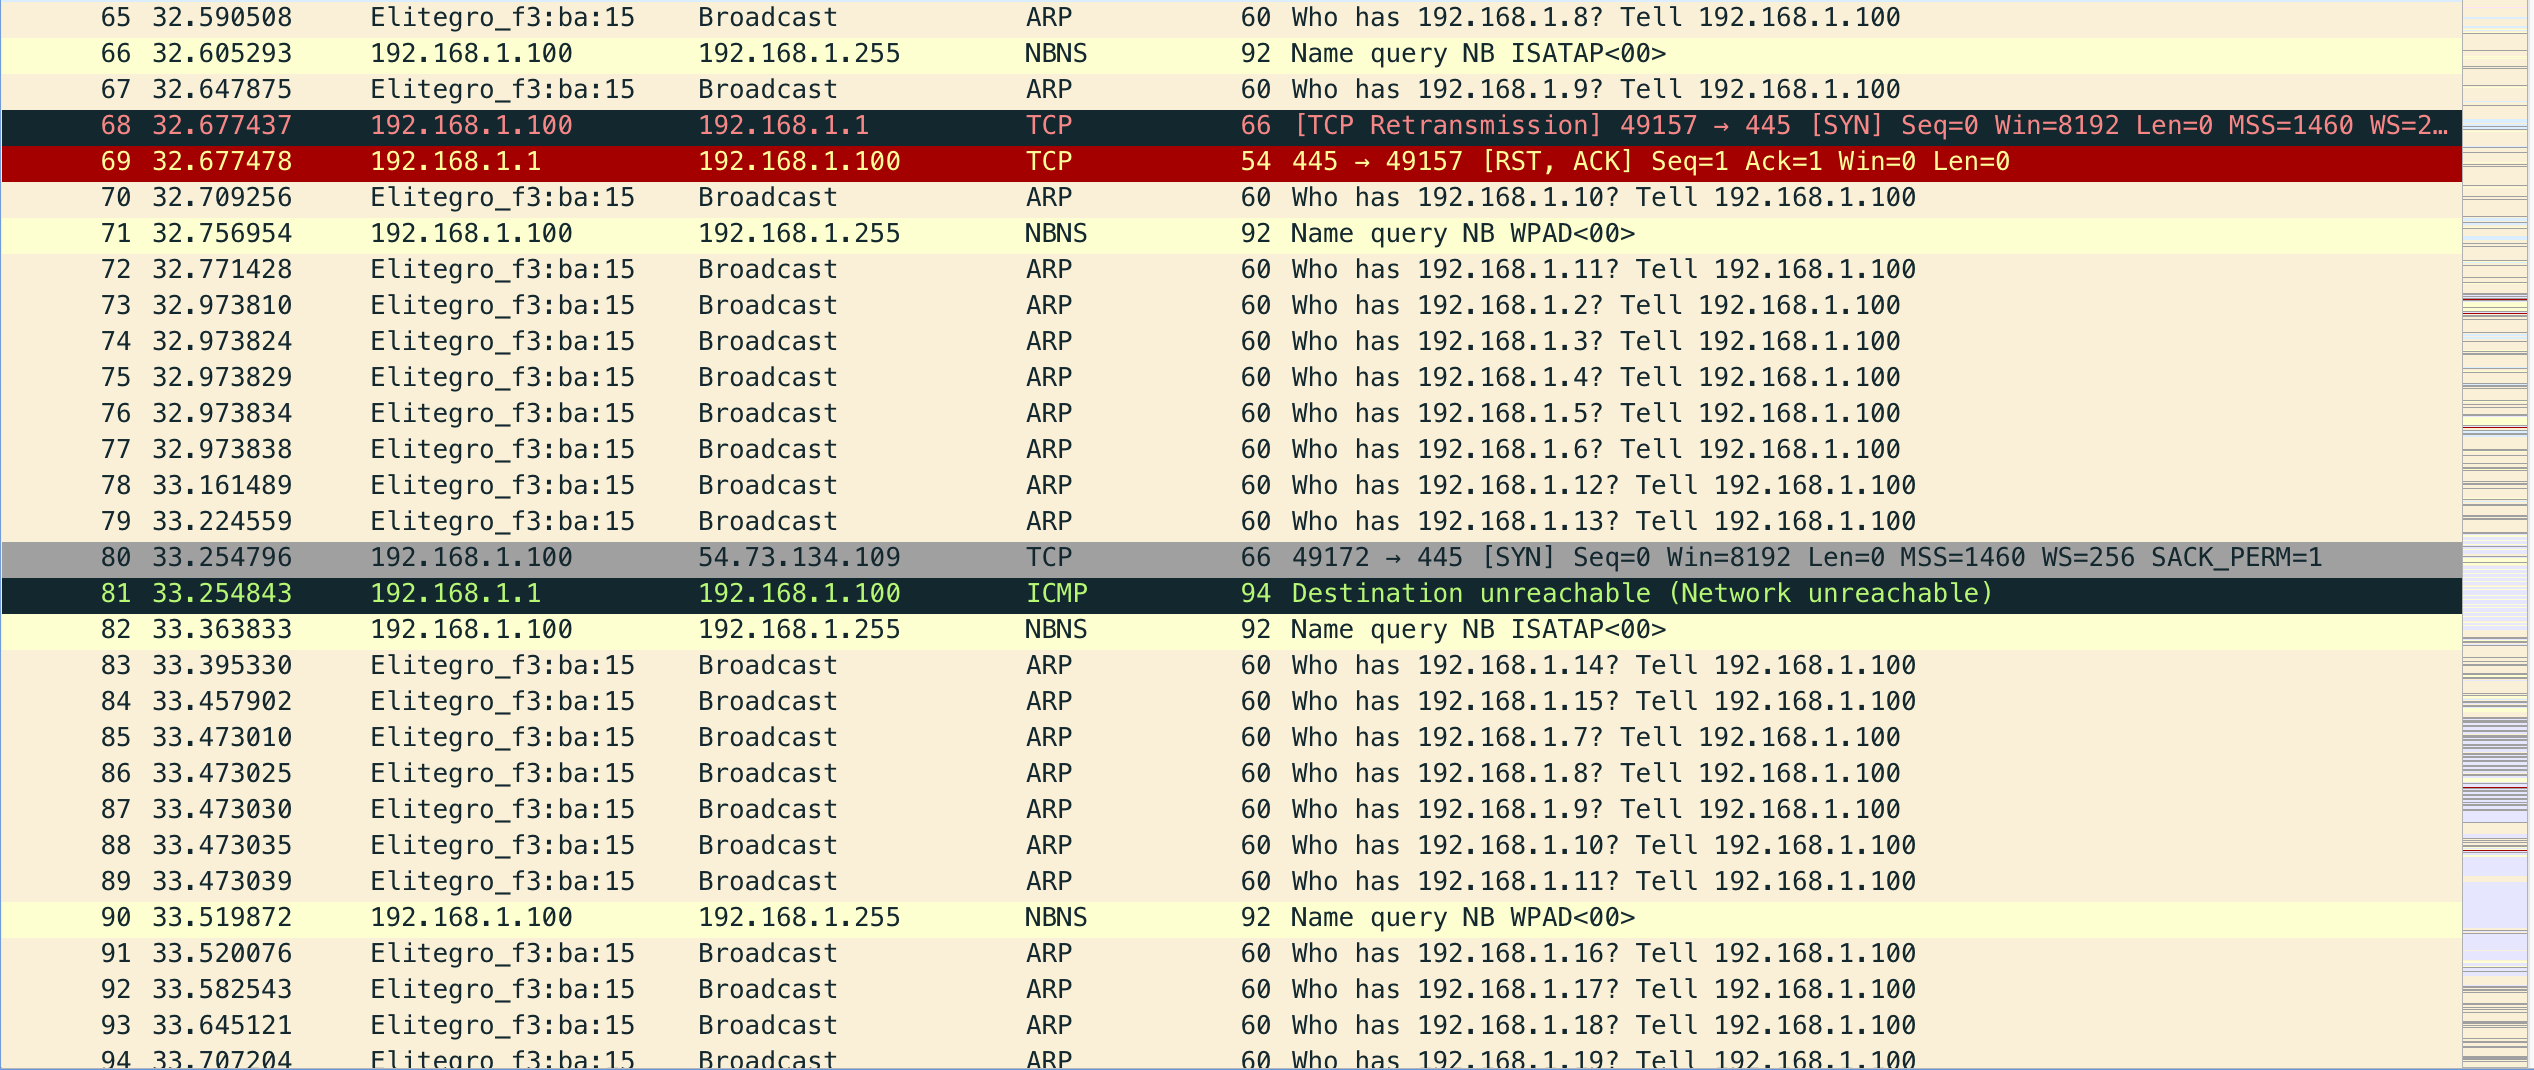
\includegraphics[width=\textwidth]{resources/infect_action.png}
	\caption{Paket pada host terinfeksi ransomware dengan dropper}
	\label{fig:infect_action}
\end{figure}

Ransomware merupakan kategori malicious software yang ketika dijalankan akan menonaktifkan fungsi tertentu dari komputer dengan sebuah cara. Kemudian ransomware akan menampilkan pesan untuk meminta pembayaran untuk mengembalikan fungsi yang dinonatifkan. Sehingga malware seakan-akan melakukan penyandraan terhadap komputer. (\cite{o2012ransomware}).

\section{Analisis Payload SMB oleh WannaCry}

Dari riset yang telah dilakukan oleh \cite{islam2018smb}, WannaCry melakukan exploit terhadap vulnerability yang menurut EternalBlue dan DoublePulsar yang ada pada implementasi SMB1.

\subsection{Vulnerability EternalBlue}
EternalBlue merupakan vulnerability yang diakibatkan oleh 3 buah bug (\cite{islam2018smb}) dan (\cite{grossman2017check}) yakni:
\begin{enumerate}
	\item Wrong casting bug
	\item Wrong parsing function bug
	\item Non-paged pool allocation bug
\end{enumerate}

Pada host 192.168.1.100 paket yang dikirimkan malware untuk mengeksploitasi vulnerability seperti yang disebutkan (\cite{islam2018smb}), yakni dengan mengirimkan \verb|SMB_COM_NT_TRANSACT| terlihat pada Gambar \ref{fig:trans_nop}, diikuti dengan \verb|SMB_COM_TRANSACTION2_SECONDARY| seperti pada Gambar \ref{fig:trans2_secondary}.

\begin{figure}[H]
	\centering
	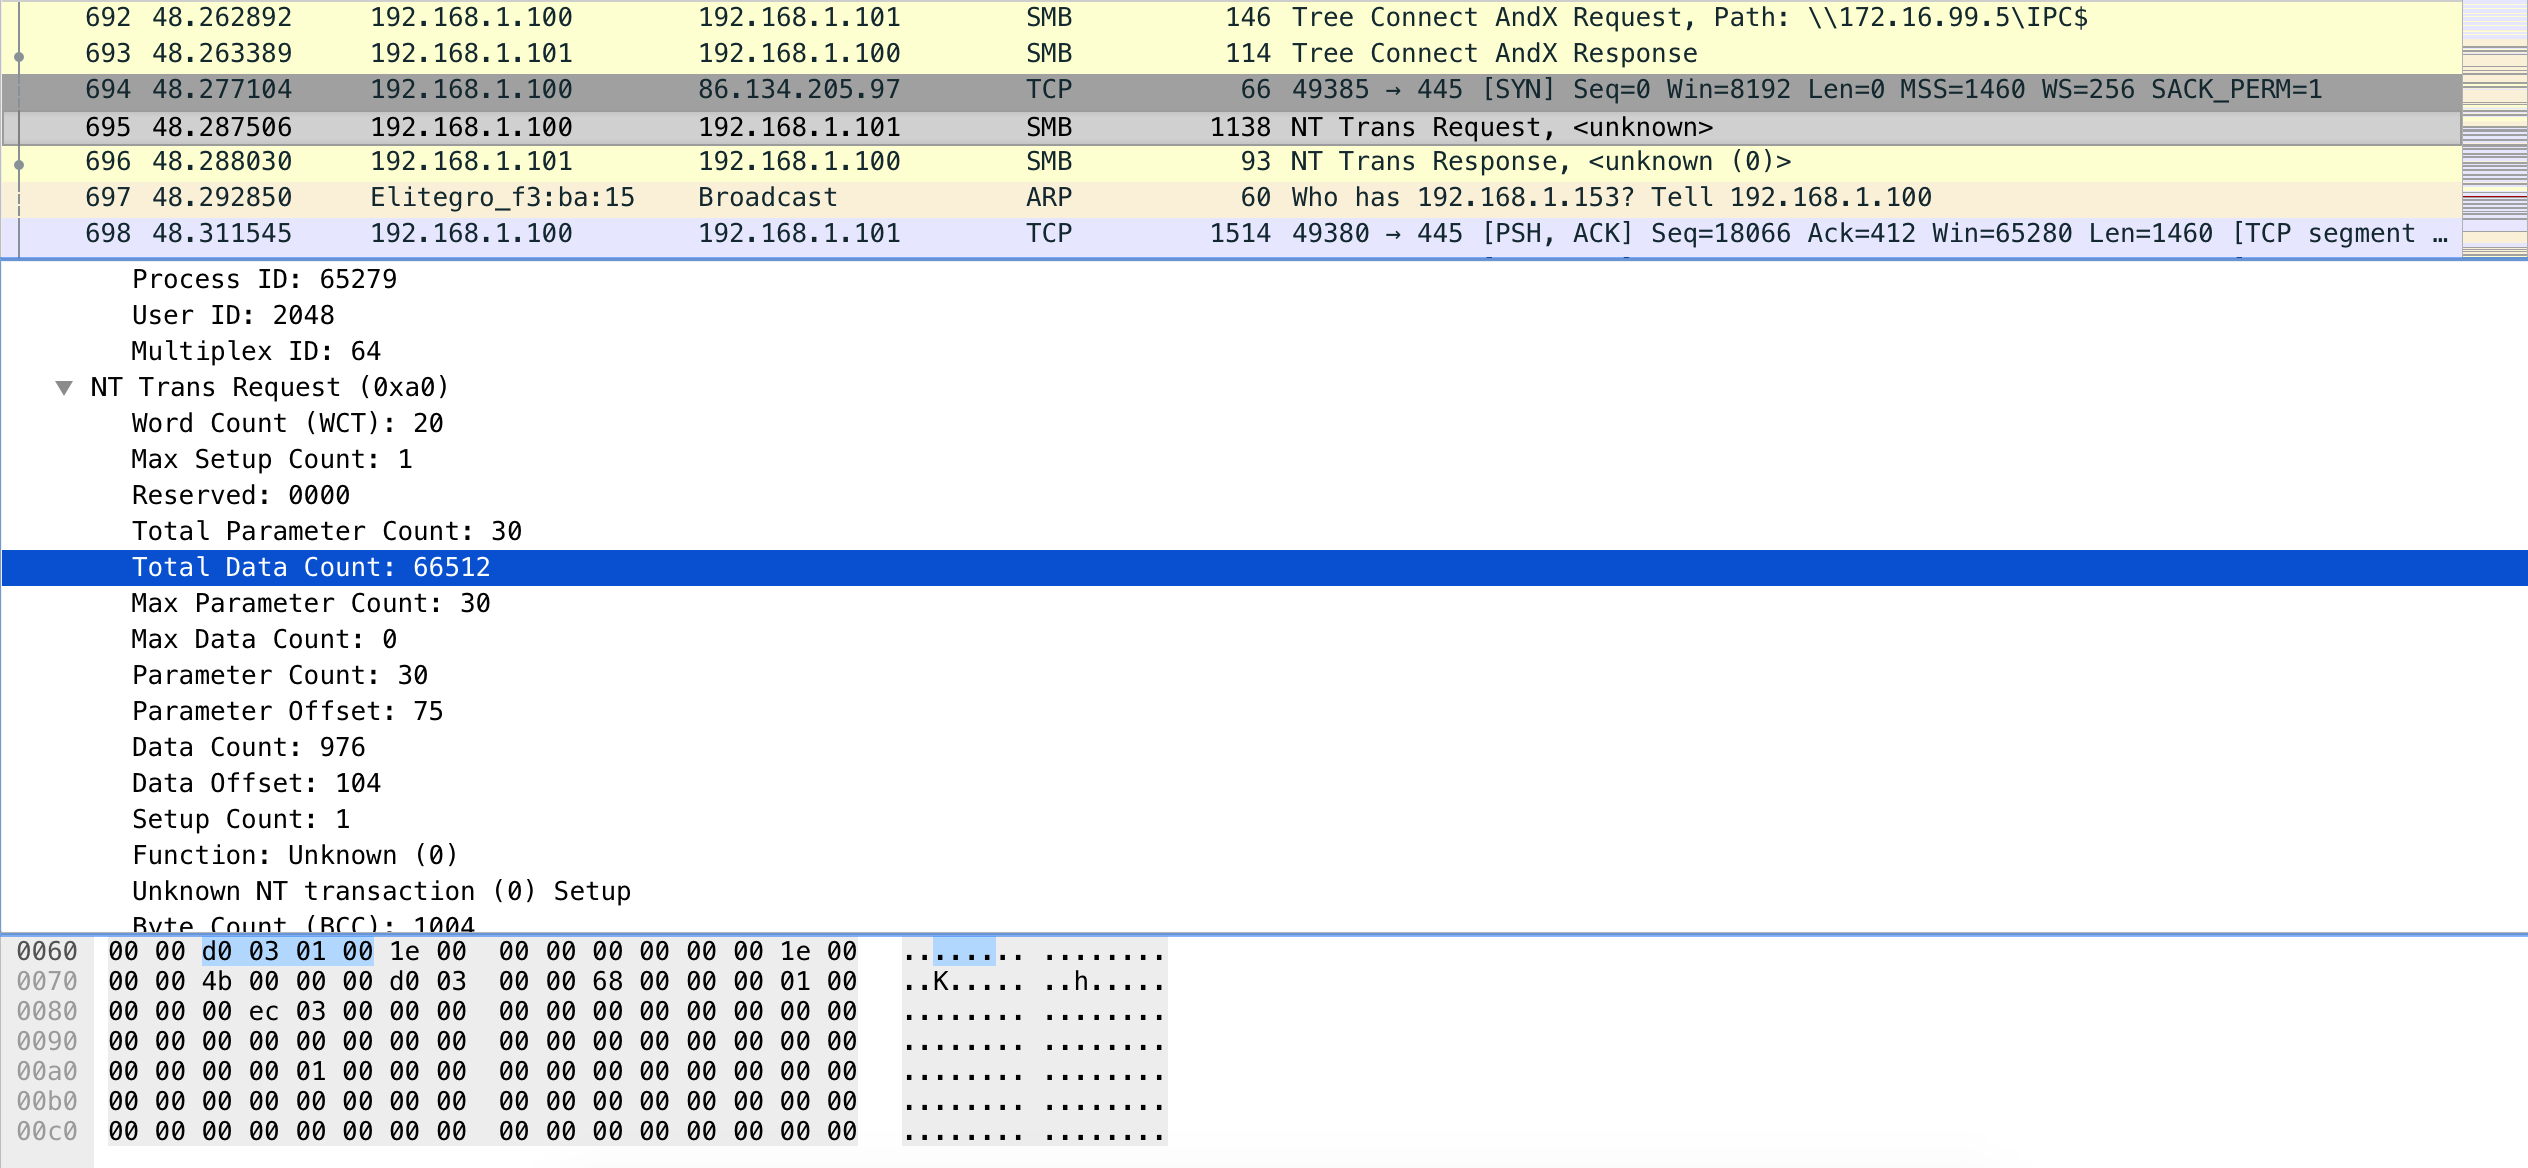
\includegraphics[width=\textwidth]{resources/trans_nop.png}
	\caption{Paket SMB\_COM\_NT\_TRANSACT dari host terinfeksi}
	\label{fig:trans_nop}
\end{figure}
\begin{figure}[H]
	\centering
	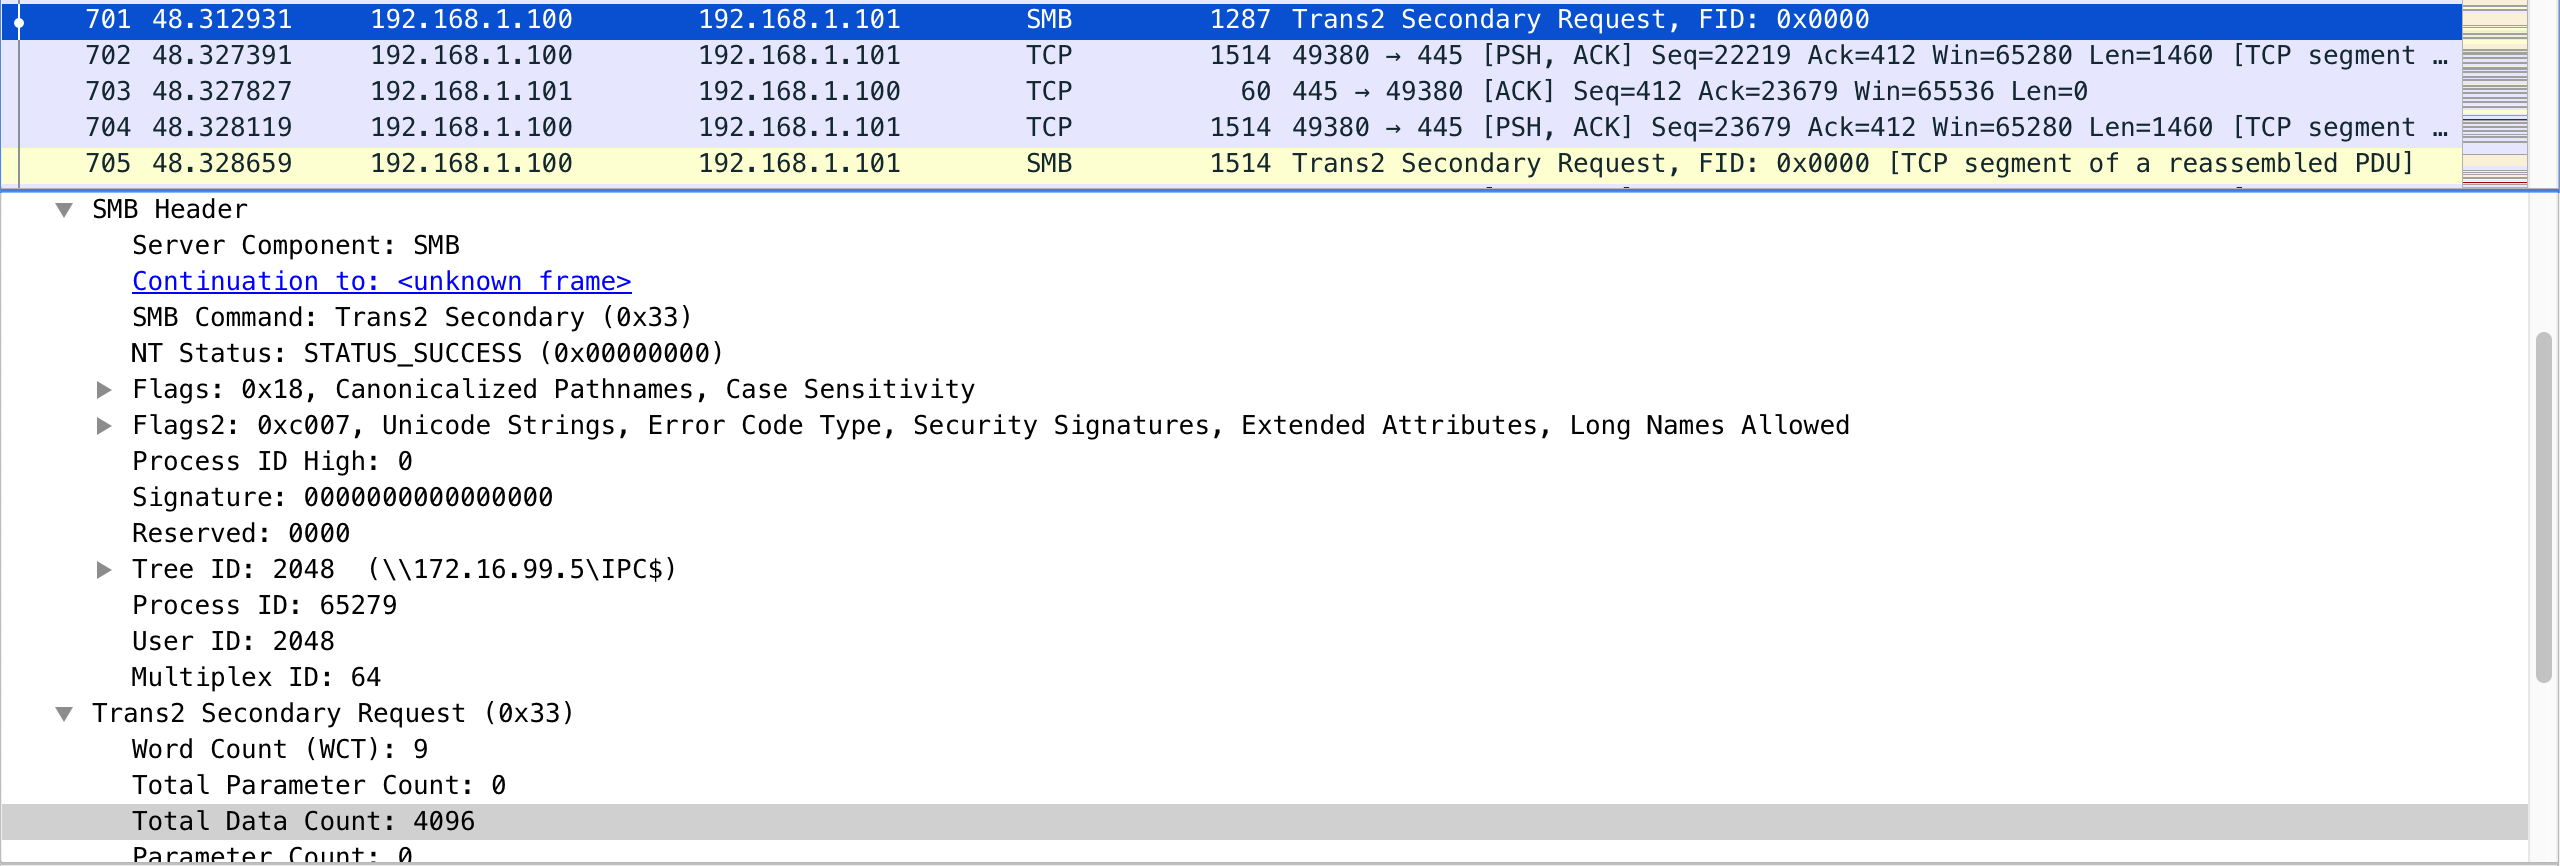
\includegraphics[width=\textwidth]{resources/trans2_secondary.png}
	\caption{Paket SMB\_COM\_TRANSACTION2\_SECONDARY dari host terinfeksi}
	\label{fig:trans2_secondary}
\end{figure}

\subsection{Vulnerability DoublePulsar}


Pada malware wannacry

\section{Deteksi Protokol}
Untuk membuat sebuah firewall yang dapat melakukan block terhadap payload malicious yang dikirim oleh WannaCry, firewall harus dapat membedakan jenis paket. Penentuan jenis paket ini dapat dilakukan dengan melakukan inspeksi paket yang merupakan fitur dari DPI (Deep Packet Inspection).

\subsection{OpenDPI}
Menurut (\cite{khalife2013performance}), OpenDPI merupakan salah satu kakas yang merupakan turunan dari produk PACE dari Ipoque. OpenDPI pada awalnya dikembangkan untuk melakukan deteksi dan mengatur lalu lintas data peer-to-peer dengan melakukan inspeksi paket. OpenDPI pada intinya merupakan library yang didesain untuk melakukan klasifikasi pada lalu lintas data berdasarkan protokol aplikasi yang digunakan.

\subsection{nDPI}

Menurut (\cite{deri2014ndpi}), nDPI merupakan superset dari 


* The OpenDPI library is written in C and it is divided in two main components: the core library (responsible for handling raw packets, decoding IP layers 3 and 4, and extracting basic information such as IP address and port) and plugin dissectors (responsible for detecting the ~100 protocols supported by OpenDPI). nDPI inherited this two-layer architecture but it addressed several issues present in the OpenDPI design: 

* The OpenDPI library was designed to be extensible, but in practice the data structures used internally were static. For instance, many data-types and bitmaps, used to keep the state for all supported protocols, were bound to specific sizes (e.g., 128 bits) and thus limiting the number of identifiable protocols. 

* Whenever a protocol was detected, the library tried to find further protocol matches instead of just returning the first match. The result was a performance penalty without a real need of requiring extra detection work. 

* No encrypted protocol support (e.g., HTTPS). While encryption is designed to preserve privacy and regular DPI libraries are not expected to decode the some information can be gleaned to suggest the nature of the information carried on a specific connection. 

* OpenDPI was not designed to be a reentrant (i.e., thread-safe) library as it used shared global variables. This required multi-threaded applications to create several instances of the library or add semaphores in order to avoid multiple threads to modify the same data at the same time. Per thread library state was required to support reentrancy. 

* Many parts of OpenDPI suggest problematic design choices. For instance, the library was performing per- flow initializations, instead of doing them at once. As the result, the applications using the library paid an unnecessary performance penalty whenever a new connection was passed to OpenDPI. 

* The protocol dissection was non-hierarchical. In other words, whenever a new connection needed to be analyzed, the library was not applying the dissectors based on their matching probability. For instance, if there is a connection on TCP port 80, OpenDPI was not trying the HTTP dissector first, but it was applying dissectors in the same order as they were registered in the library. 

* The library had no runtime configuration capability; the only way to define new dissectors was to code them in C. While this is usually a good policy for efficiency reasons, at times more flexibility is needed. For instance, if a given user needs to define a custom protocol Y as TCP/port-X it would be easier to have a runtime configuration directive instead of changing the library code. OpenDPI assumes that the library must have a dissector for all supported protocols, a difficult goal to achieve in reality. In particular, in closed-environments such as a LAN, specific hosts use proprietary/custom protocols that flow on specific ports/protocols. In this case, it is more convenient for the user to detect them from the packet header rather than from its payload. 

* OpenDPI was not designed to extract any metadata from analyzed traffic. On one hand this preserves privacy, but on the other it requires monitoring appli- cations to decode the application traffic again in order to extract basic information such as the URL from HTTP traffic. Reporting this information does not add any overhead to the library as it is decoded anyway when parsing the packet payload. 

Summarizing, OpenDPI was a good starting point for nDPI, because we did not have to start from scratch. Many compo- nents of the original library were changed in order to address the issues we identified. This was the ground work necessary to start the creation of an efficient DPI library and extending the set of supported protocols. Not surprisingly, the number of protocols recognized has an impact on both DPI detection performance and protocol recognition. The more protocols recognized, the more time spent on detection whenever a specific traffic pattern is not identified and thus all the possible protocol decoders have to be tested for match. This means that DPI libraries supporting many protocols may be slower in specific situation than those supporting fewer. Another impact on performance is due to metadata extraction: the richer the set of extracted attributes, the slower the processing. Although specific activities such as string and pattern matching can be accelerated on specialized hardware platforms such as Cavium and RMI, or using GPUs [26], we decided not to use any of these cards, in order to let the library operate on all hardware platforms. 
nDPI was designed to be used by applications that need to detect the application protocol of communication flow. Its focus is on Internet traffic, thus all the available dissectors support standard protocols (e.g., HTTP and SMTP) or selected proprietary ones (e.g., Skype or Citrix) that are popular across the Internet community. In the latter case, as protocol specifica- tions are not publicly available, we had to create the dissectors by reverse-engineering network traffic. Although nDPI can extract specific metadata (e.g., HTTP URL) from analyzed traffic, it was not designed as a library to be used in fields such as lawful interception or data leak prevention; its primary goal is to characterize network traffic. Similarly to OpenDPI, nDPI can be used both inside the Linux kernel and in user- space applications, and it work on most operating systems including Linux, Windows, MacOS X, as well as non-Intel CPU architectures such as ARM and MIPS. 


\section{Deteksi signature dengan string matching}


\section{Penangkalan paket \textit{malicious} dengan firewall}


\section{Penentuan rule iptables untuk melakukan \textit{block} pada \textit{payload} WannaCry}


